\documentclass{article}
\usepackage[margin=1.5cm]{geometry}
\usepackage{graphicx}
\graphicspath{ {./figs/} }
\usepackage[hidelinks]{hyperref}
\setlength\parindent{0pt}

\usepackage{array }% New env. for equation conditions where aligned
\newenvironment{conditions}[1][where:] 
  {#1 \begin{tabular}[t]{>{$}l<{$} @{${}={}$} l}}
  {\end{tabular}\\[\belowdisplayskip]}

\usepackage{tikz}
\usepackage{pgfplots}

\title{Kriging Notes}

\begin{document}
\maketitle

\section{Introduction}

\begin{center}
    \fbox{Information from \href{https://desktop.arcgis.com/en/arcmap/10.3/tools/3d-analyst-toolbox/how-kriging-works.htm}{ARCGIS}}
\end{center}

Kriging is a way to interpolate data and estimate a surface for geospatial data.
There are two main ways of doing this:

\begin{itemize}
    \item Inverse distance weighting (IDW) and spline methods
    \item Kriging
\end{itemize}

IDW are deterministic interpolation methods as they are directly based on the surrounding values or smoothed formulas.
Kriging is different as it uses autocorrelation and takes position into account in the statistical models.
Kriging uses a certain number of neighbouring points, or all points within a specified radius (cf kNN).

The general formula for IDW and kriging is:

\[\hat{Z}\left(s_{0} \right)=\sum_{i=1}^{N}\lambda_{i} Z \left(s_{i}\right)\]

\begin{conditions}
Z \left(s_{i}\right) & the measured value at the $i$th location \\
\lambda_{i} & an unknown weight for the measured value at the $i$th location \\
s_{0} & the prediction location \\
N & the number of measured values
\end{conditions}

The difference between IDW and kriging is that in IDW, $\lambda_{i}$ only depends on distance to prediction location.
In kriging $\lambda_{i}$ also depends on autocorrelation i.e. spatial relationship between prediction locations.

\section{Creating a prediction map with kriging}

There are two steps:

\begin{enumerate}
    \item Create the variograms and covariance functions to estimate the spatial autocorrelation values that depend on the model of autocorrelation (fitting a model).
    \item Predict the unknown values
\end{enumerate}

\subsection{Variography (spatial modelling/structural analysis)}

There are often too many pairs of spatial points to calculate and plot the distance for each pair.
Instead, spatial distances are put into lag bins i.e. all points in the range $40m < x \le 50m$ of point A, and calculate the semivariance.
The semivariance is equal to half the variance of the differences between all possible points spaced a constant distance apart.

\[\gamma (h) = \frac{1}{2}\left[z(x_{i}) - z(x_{j})\right]^2\]

Plotting the distance vs semivariance produces an empirical semivariogram.
Closer items should be more similar, therefore lower semivariance.
The opposite is true for further points.

A model is fit to the empirical semivariogram (cf regression).
Different types of models can be fit the the semivariogram:

\begin{itemize}
    \item Spherical (most common)
    \item Circular
    \item Exponential
    \item Gaussian
    \item Linear
\end{itemize}

\begin{center}
    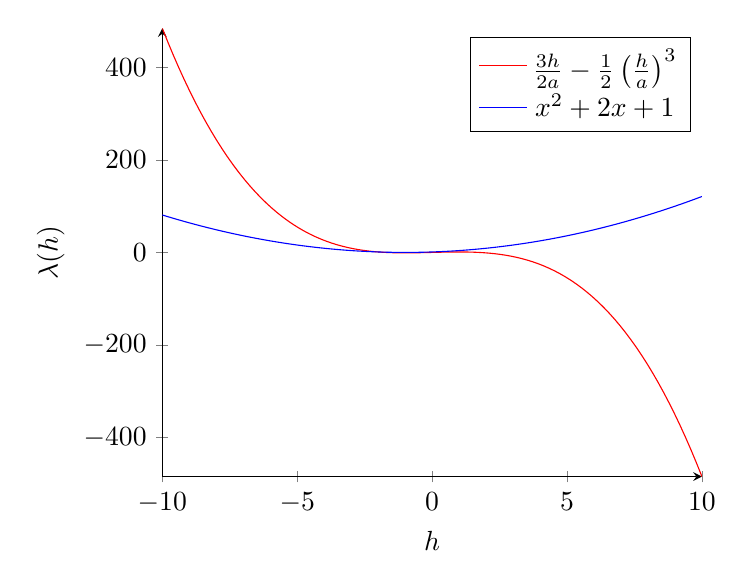
\begin{tikzpicture}
        \begin{axis}[
            axis lines = left,
            xlabel = $h$,
            ylabel = {$\lambda(h)$},
        ]
        %Below the red parabola is defined
        \addplot [
            domain=-10:10, 
            samples=100, 
            color=red,
        ]
        {3*x/2 - 1/2 * x^3};
        \addlegendentry{$\frac{3h}{2a} - \frac{1}{2}\left(\frac{h}{a}\right)^3$}
        %Here the blue parabloa is defined
        \addplot [
            domain=-10:10, 
            samples=100, 
            color=blue,
            ]
            {x^2 + 2*x + 1};
        \addlegendentry{$x^2 + 2x + 1$}
        
        \end{axis}
    \end{tikzpicture}
\end{center}


\end{document}